
\section{Pianificazione}
\subsection{Modello adottato}

COPIA QUELLO DI BYTEOPS

\subsection{Periodi}

Per ogni periodo si riportano di seguito le seguenti informazioni:
\begin{itemize}
    \item data di inizio, data di fine prevista, data di fine attuale ed eventuali giorni di ritardo;
    \item pianificazione delle attività da svolgere al suo interno (avanzamento atteso), con tanto di potenziali rischi;
    \item tempo stimato per poter completare tutte le attività previste;
    \item confronto fra il lavoro svolto (avanzamento conseguito) e quello preventivato, con annessa analisi dei costi;
    \item rischi effettivamente occorsi, valutandone il loro impatto e la loro mitigazione;
    \item retrospettiva di periodo per capire cosa e come migliorare in futuro e cosa invece mantenere;
\end{itemize}
I periodi vengono suddivisi in 3 grandi insiemi corrispondenti alle revisioni di avanzamento del progetto:
\begin{itemize}
    \item \textbf{RTB}: \textit{\textbf{R}equirements and \textbf{T}echnology \textbf{B}aseline};
    \item \textbf{PB}:  \textit{\textbf{P}roduct\textbf{B}aseline};
    \item \textbf{CA}:  \textit{\textbf{C}ustomer \textbf{A}cceptance}.
\end{itemize}

\subsection{Requirements and Technology Baseline}
    \subsubsection{Primo sprint:}
        \begin{itemize}
            \item Inizio: 03/04/2024
            \item FIne: 19/04/2024
            \item Fine attuale: 
            \item Giorni di ritardo: 
        \end{itemize}
        \subsubsubsection{Pianificazione} 
        Durante questo periodo, il team si concentra sul dedicare risorse significative allo sviluppo, alla standardizzazione e all'automazione dei processi, ove possibile. Nel primo incontro con l'azienda proponente vengono definiti gli obiettivi chiave da raggiungere entro il prossimo SAL del 19 aprile 2024. \\In particolare, questi obiettivi comprendono:
        \begin{itemize}
            \item simulazione di un sensore mediante codice Python;
            \item integrazione con server Apache Kafka utilizzando ambiente Docker;
            \item USER STORY E CASI D'USO CORRELATI AL CAPITOLATO
        \end{itemize}

        Parallelamente a questa fase, l'amministratore ha stanziato risorse per automatizzare il processo di compilazione dei sorgenti LateX una volta caricati sul repository condiviso, e per distinguere automaticamente le parole presenti nel glossario da quelle che non lo sono.

        \subsubsubsubsection{Rischi attesi}
        I rischi attesi per questo periodo sono:
        \begin{itemize}
            \item inesperienza del team (Rischio RT2);
            \item imprecisione nella pianificazione delle attività (Rischio RO3);
            \item elevati costi delle attività (Rischio RO3);
            \item rischio di conflitti interni (Rischio RC1);
            \item problemi di comunicazione (Rischio RC2).
        \end{itemize}
        Ciò è causato dal fatto che, poiché siamo ancora all'inizio del progetto, non abbiamo ancora una chiara idea di come organizzarci per massimizzare l'uso del tempo e delle risorse.
        \newpage
        \subsubsubsection{Preventivo}
        Ruoli coinvolti: Amministratore, Responsabile, Verificatore, Analista, Programmatore.

        \begin{table}[!h]
            \centering
            \begin{tabular}{ |l| c| c| c| c| c| } 
                \hline
                \textbf{} & \textbf{Amministratore} & \textbf{Responsabile} & \textbf{Verificatore} &\textbf{Analista} & \textbf{Programmatore} \\
                \hline 
                Tiozzo      & 0 & 0 & 0 & 0 & 0 \\ 
                Malgarise   & 0 & 0 & 0 & 0 & 0 \\ 
                Ferro       & 0 & 0 & 0 & 0 & 0 \\ 
                Benetazzo   & 0 & 0 & 0 & 0 & 0 \\ 
                Occhinegro  & 0 & 0 & 0 & 0 & 0 \\ 
                Baldo       & 0 & 0 & 0 & 0 & 0 \\ 
                Seganfreddo & 0 & 0 & 0 & 0 & 0 \\
                \hline
            \end{tabular}
            \caption{Preventivo orario per ruolo di ciascun membro del team durante il primo sprint}
            \label{tab:1}
        \end{table}


%---------1_ISTOGRAMMA-----------%
        \begin{figure*}
            \centering
            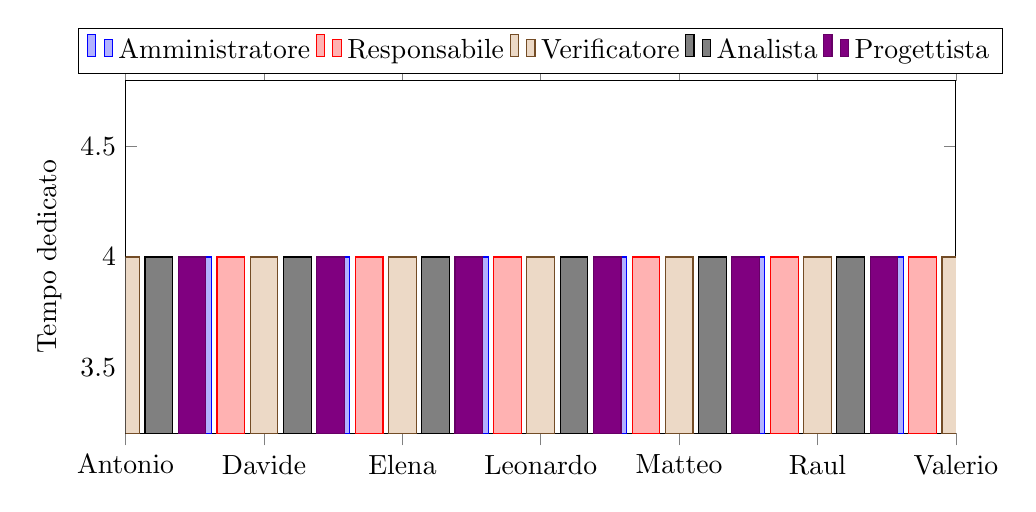
\begin{tikzpicture}
                \begin{axis}[
                    width=\textwidth,
                    height=0.5\textwidth,
                    ybar,
                    enlargelimits=0,
                    legend style={at={(0.5,1.15)},
                      anchor=north,legend columns=-1},
                    ylabel={Tempo dedicato},    
                    symbolic x coords={Antonio, Davide, Elena, Leonardo, Matteo, Raul, Valerio},
                    xtick=data,
                    % nodes near coords,
                    nodes near coords align={vertical},
                    ]
                \addplot coordinates {(Antonio,4) (Davide,4) (Elena,4) (Leonardo,4) (Matteo,4) (Raul,4) (Valerio,4)};
                \addplot coordinates {(Antonio,4) (Davide,4) (Elena,4) (Leonardo,4) (Matteo,4) (Raul,4) (Valerio,4)};
                \addplot coordinates {(Antonio,4) (Davide,4) (Elena,4) (Leonardo,4) (Matteo,4) (Raul,4) (Valerio,4)};
                \addplot coordinates {(Antonio,4) (Davide,4) (Elena,4) (Leonardo,4) (Matteo,4) (Raul,4) (Valerio,4)};
                \addplot coordinates {(Antonio,4) (Davide,4) (Elena,4) (Leonardo,4) (Matteo,4) (Raul,4) (Valerio,4)};
                \legend{Amministratore, Responsabile, Verificatore, Analista, Progettista}
                \end{axis}
            \end{tikzpicture}
        \caption{Impegno preventivo per ruolo di ciascun membro del team durante il primo periodo}
        \label{fig:1}
        \end{figure*}

        \newblock
%---------1_GRAFICO A TORTA-----------%
        \begin{figure*}
        \centering
        \begin{tikzpicture}
            \pie[rotate=90, text=legend]{
                20/Verificatore,
                20/Analista,
                20/Amministratore,
                20/Responsabile,
                20/Progettista
            }
        \end{tikzpicture}
        \caption{Ripartizione in percentuale dei ruoli nel primo periodo}
        \label{fig:2}
        \end{figure*}


        \newblock
        \newpage

        \subsubsubsection{Consuntivo}
        Le attività previste sono state tutte svolte con successo. Come si può vedere dal confronto tra preventivo e consuntivo:
        \begin{itemize}
            \item Amministratore: 0 ore preventivate, 0 ore effettive;
            \item Responsabile: 0 ore preventivate, 0 ore effettive;
        \end{itemize}
        \subsubsubsubsection{Prospetto orario}

        \begin{table}[!h]
            \centering
            \begin{tabular}{ |l| c |c |c |c |c| } 
                \hline
                \textbf{} & \textbf{Amministratore} & \textbf{Responsabile} & \textbf{Verificatore} &\textbf{Analista} & \textbf{Progettista} \\
                \hline 
                Tiozzo      & 0 & 0 & 0 & 0 & 0 \\ 
                Malgarise   & 0 & 0 & 0 & 0 & 0 \\ 
                Ferro       & 0 & 0 & 0 & 0 & 0 \\ 
                Benetazzo   & 0 & 0 & 0 & 0 & 0 \\ 
                Occhinegro  & 0 & 0 & 0 & 0 & 0 \\ 
                Baldo       & 0 & 0 & 0 & 0 & 0 \\ 
                Seganfreddo & 0 & 0 & 0 & 0 & 0 \\
                \hline
            \end{tabular}
            \caption{Impegno effettivo per ruolo di ciascun membro del team durante il primo periodo}
            \label{tab:2}
        \end{table}
        \newpage
        \subsubsubsubsection{Prospetto economico}

        \begin{table}[!h]
            \centering
            \begin{tabular}{|l| c| c| c| c| c| } 
                \hline
                \textbf{} & \textbf{Ruolo} & \textbf{Ore} & \textbf{Costo} &\textbf{Differenza} \\
                \hline  
                 & Responsabile        & 0 & 0 & 0 \\ 
                 & Amministratore      & 0 & 0 & 0 \\ 
                 & Verificatore        & 0 & 0 & 0 \\ 
                 & Analista            & 0 & 0 & 0 \\ 
                 & Progettista         & 0 & 0 & 0 \\ 
                 & Programmatore       & 0 & 0 & 0 \\ 
                 & Seganfreddo         & 0 & 0 & 0 \\
                Totale preventivo & - & 0 & 0 &0 \\
                Totale consuntivo & - & 0 & 0 & 0\\
                \hline
            \end{tabular}
            \caption{Aggiornamenti economici del progetto al termine del primo periodo, riflettendo le variazioni tra preventivo e ore effettivamente lavorate}
            \label{tab:3}
        \end{table}
        \subsubsubsubsection{Rischi effettivamente occorsi e loro mitigazione}
        SCRITTURA DEI RISCHI CHE ABBIAMO TROVATO DURANTE QUESTO PRIMO PERIODO E COME LI ABBIAMO RISOLTI
        \subsubsubsection{Retrospettiva}
        SCRITTURA DI COSA ABBIAMO FATTO BENE E COSA ABBIAMO SBAGIATO, COSÌ DA MIGLIORARCI
\newpage
    \subsubsection{Secondo sprint:}
    \begin{itemize}
        \item Inizio: 10/04/2024
        \item FIne: 24/04/2024
        \item Fine attuale:
        \item Giorni di ritardo:
    \end{itemize}
    \subsubsubsection{Pianificazione} 
    SCRIVI QUALCOSA A RIGUARDO (PT. 4.1.1.1 DEGLI OVERTURE)
    \subsubsubsubsection{Rischi attesi}
    I rischi attesi per questo periodo sono:
    \begin{itemize}
        \item Inesperienza del team
        \item Imprecisione nella pianificazione delle attività
        \item Elevati costi delle attività
        \item Rischio di conflitti interni 
        \item problemi di comunicazione
        \item problemi di coordinamento
    \end{itemize}
    Questo perchè, essendo all’inizio del progetto, siamo ancora incerti su molti aspetti di quest’ultimo, ci stiamo attualmente organizzando e dobbiamo apprendere ancora molto, dunque la probabilità di incorrere in qualche problema tra quelli riportati è abbastanza elevata.
    \subsubsubsection{Preventivo}
    Ruoli coinvolti: 
    \subsubsubsection{Consuntivo}
    Le attività previste sono state tutte svolte con successo
    \subsubsubsubsection{Prospetto orario}
    \subsubsubsubsection{Prospetto economico}
    \subsubsubsubsection{Rischi effettivamente occorsi e loro mitigazione}
    \subsubsubsection{Retrospettiva}


    \subsubsection{Terzo sprint:}
    \begin{itemize}
        \item Inizio: 25/04/2024
        \item FIne: 09/05/2024
        \item Fine attuale:
        \item Giorni di ritardo:
    \end{itemize}
    \subsubsubsection{Pianificazione} 
    SCRIVI QUALCOSA A RIGUARDO (PT. 4.1.1.1 DEGLI OVERTURE)
    \subsubsubsubsection{Rischi attesi}
    I rischi attesi per questo periodo sono:
    \begin{itemize}
        \item Inesperienza del team
        \item Imprecisione nella pianificazione delle attività
        \item Elevati costi delle attività
        \item Rischio di conflitti interni 
        \item problemi di comunicazione
        \item problemi di coordinamento
    \end{itemize}
    Questo perchè, essendo all’inizio del progetto, siamo ancora incerti su molti aspetti di quest’ultimo, ci stiamo attualmente organizzando e dobbiamo apprendere ancora molto, dunque la probabilità di incorrere in qualche problema tra quelli riportati è abbastanza elevata.
    \subsubsubsection{Preventivo}
    Ruoli coinvolti: 
    \subsubsubsection{Consuntivo}
    Le attività previste sono state tutte svolte con successo
    \subsubsubsubsection{Prospetto orario}
    \subsubsubsubsection{Prospetto economico}
    \subsubsubsubsection{Rischi effettivamente occorsi e loro mitigazione}
    \subsubsubsection{Retrospettiva}

    \subsubsection{Quarto sprint:}
    \begin{itemize}
        \item Inizio: 10/05/2024
        \item FIne: 24/05/2024
        \item Fine attuale:
        \item Giorni di ritardo:
    \end{itemize}
    \subsubsubsection{Pianificazione} 
    SCRIVI QUALCOSA A RIGUARDO (PT. 4.1.1.1 DEGLI OVERTURE)
    \subsubsubsubsection{Rischi attesi}
    I rischi attesi per questo periodo sono:
    \begin{itemize}
        \item Inesperienza del team
        \item Imprecisione nella pianificazione delle attività
        \item Elevati costi delle attività
        \item Rischio di conflitti interni 
        \item problemi di comunicazione
        \item problemi di coordinamento
    \end{itemize}
    Questo perchè, essendo all’inizio del progetto, siamo ancora incerti su molti aspetti di quest’ultimo, ci stiamo attualmente organizzando e dobbiamo apprendere ancora molto, dunque la probabilità di incorrere in qualche problema tra quelli riportati è abbastanza elevata.
    \subsubsubsection{Preventivo}
    Ruoli coinvolti: 
    \subsubsubsection{Consuntivo}
    Le attività previste sono state tutte svolte con successo
    \subsubsubsubsection{Prospetto orario}
    \subsubsubsubsection{Prospetto economico}
    \subsubsubsubsection{Rischi effettivamente occorsi e loro mitigazione}
    \subsubsubsection{Retrospettiva}

    \subsubsection{Quinto sprint:}
    \begin{itemize}
        \item Inizio: 25/05/2024
        \item FIne: 09/06/2024
        \item Fine attuale:
        \item Giorni di ritardo:
    \end{itemize}
    \subsubsubsection{Pianificazione} 
    SCRIVI QUALCOSA A RIGUARDO (PT. 4.1.1.1 DEGLI OVERTURE)
    \subsubsubsubsection{Rischi attesi}
    I rischi attesi per questo periodo sono:
    \begin{itemize}
        \item Inesperienza del team
        \item Imprecisione nella pianificazione delle attività
        \item Elevati costi delle attività
        \item Rischio di conflitti interni 
        \item problemi di comunicazione
        \item problemi di coordinamento
    \end{itemize}
    Questo perchè, essendo all’inizio del progetto, siamo ancora incerti su molti aspetti di quest’ultimo, ci stiamo attualmente organizzando e dobbiamo apprendere ancora molto, dunque la probabilità di incorrere in qualche problema tra quelli riportati è abbastanza elevata.
    \subsubsubsection{Preventivo}
    Ruoli coinvolti: 
    \subsubsubsection{Consuntivo}
    Le attività previste sono state tutte svolte con successo
    \subsubsubsubsection{Prospetto orario}
    \subsubsubsubsection{Prospetto economico}
    \subsubsubsubsection{Rischi effettivamente occorsi e loro mitigazione}
    \subsubsubsection{Retrospettiva}


    \subsubsection{Sesto sprint:}
    \begin{itemize}
        \item Inizio: 10/06/2024
        \item FIne: 24/06/2024
        \item Fine attuale:
        \item Giorni di ritardo:
    \end{itemize}
    \subsubsubsection{Pianificazione} 
    SCRIVI QUALCOSA A RIGUARDO (PT. 4.1.1.1 DEGLI OVERTURE)
    \subsubsubsubsection{Rischi attesi}
    I rischi attesi per questo periodo sono:
    \begin{itemize}
        \item Inesperienza del team
        \item Imprecisione nella pianificazione delle attività
        \item Elevati costi delle attività
        \item Rischio di conflitti interni 
        \item problemi di comunicazione
        \item problemi di coordinamento
    \end{itemize}
    Questo perchè, essendo all’inizio del progetto, siamo ancora incerti su molti aspetti di quest’ultimo, ci stiamo attualmente organizzando e dobbiamo apprendere ancora molto, dunque la probabilità di incorrere in qualche problema tra quelli riportati è abbastanza elevata.
    \subsubsubsection{Preventivo}
    Ruoli coinvolti: 
    \subsubsubsection{Consuntivo}
    Le attività previste sono state tutte svolte con successo
    \subsubsubsubsection{Prospetto orario}
    \subsubsubsubsection{Prospetto economico}
    \subsubsubsubsection{Rischi effettivamente occorsi e loro mitigazione}
    \subsubsubsection{Retrospettiva}

    \subsubsection{Settimo sprint:}
    \begin{itemize}
        \item Inizio: 25/06/2024
        \item FIne: 09/07/2024
        \item Fine attuale:
        \item Giorni di ritardo:
    \end{itemize}
    \subsubsubsection{Pianificazione} 
    SCRIVI QUALCOSA A RIGUARDO (PT. 4.1.1.1 DEGLI OVERTURE)
    \subsubsubsubsection{Rischi attesi}
    I rischi attesi per questo periodo sono:
    \begin{itemize}
        \item Inesperienza del team
        \item Imprecisione nella pianificazione delle attività
        \item Elevati costi delle attività
        \item Rischio di conflitti interni 
        \item problemi di comunicazione
        \item problemi di coordinamento
    \end{itemize}
    Questo perchè, essendo all’inizio del progetto, siamo ancora incerti su molti aspetti di quest’ultimo, ci stiamo attualmente organizzando e dobbiamo apprendere ancora molto, dunque la probabilità di incorrere in qualche problema tra quelli riportati è abbastanza elevata.
    \subsubsubsection{Preventivo}
    Ruoli coinvolti: 
    \subsubsubsection{Consuntivo}
    Le attività previste sono state tutte svolte con successo
    \subsubsubsubsection{Prospetto orario}
    \subsubsubsubsection{Prospetto economico}
    \subsubsubsubsection{Rischi effettivamente occorsi e loro mitigazione}
    \subsubsubsection{Retrospettiva}

    \subsubsection{Sommario finale}
    \subsubsubsection{Riepilogo prospetto orario}
    \subsubsubsubsection{Ore consumate}
    \subsubsubsubsection{Ore rimanenti}
    \subsubsubsection{Riepilogo prospetto economico}
    \subsubsubsection{Costi totali}

    \subsection{Tra RTB e PB}
    \subsubsection{Ottavo periodo}
    \begin{itemize}
        \item Inizio: 10/07/2024
        \item FIne: 24/07/2024
        \item Fine attuale:
        \item Giorni di ritardo:
    \end{itemize}
    \subsubsubsection{Pianificazione} 
    SCRIVI QUALCOSA A RIGUARDO (PT. 4.1.1.1 DEGLI OVERTURE)
    \subsubsubsubsection{Rischi attesi}
    I rischi attesi per questo periodo sono:
    \begin{itemize}
        \item Inesperienza del team
        \item Imprecisione nella pianificazione delle attività
        \item Elevati costi delle attività
        \item Rischio di conflitti interni 
        \item problemi di comunicazione
        \item problemi di coordinamento
    \end{itemize}
    Questo perchè, essendo all’inizio del progetto, siamo ancora incerti su molti aspetti di quest’ultimo, ci stiamo attualmente organizzando e dobbiamo apprendere ancora molto, dunque la probabilità di incorrere in qualche problema tra quelli riportati è abbastanza elevata.
    \subsubsubsection{Preventivo}
    Ruoli coinvolti: 
    \subsubsubsection{Consuntivo}
    \subsubsubsubsection{Prospetto orario}
    \subsubsubsubsection{Prospetto economico}
    \subsubsubsubsection{Rischi effettivamente occorsi e loro mitigazione}
    \subsubsubsection{Retrospettiva}

% \subsection{Product Baseline}


% \section{Preventivo}
% \subsection{Requirements and Technology Baseline}
%     \subsubsection{Primo sprint:}
%     \subsubsection{Secondo sprint:}
%     \subsubsection{Terzo sprint:}
%     \subsubsection{Quarto sprint:}
%     \subsubsection{Quinto sprint:}
%     \subsubsection{Sesto sprint:}
%     \subsubsection{Settimo sprint:}
% \subsection{Preventivo a finire}
%     \subsubsection{Resoconto finale RTB}
%     \subsubsection{Risuddivisione oraria}

% \section{Consuntivo}
% \subsection{Requirements and Technology Baseline}
%     \subsubsection{Primo sprint:}
%     \subsubsection{Secondo sprint:}
%     \subsubsection{Terzo sprint:}
%     \subsubsection{Quarto sprint:}
%     \subsubsection{Quinto sprint:}
%     \subsubsection{Sesto sprint:}
%     \subsubsection{Settimo sprint:}


